%%%%%%%%%%%%%%%%%%%%%%%%%%%%%%%%%%%%%%%%%%%%%%%%%%%%%%%%%%%%%%%%%%%%%%%%
%
%		Chapter 4 - Higher-Order Models
%
%%%%%%%%%%%%%%%%%%%%%%%%%%%%%%%%%%%%%%%%%%%%%%%%%%%%%%%%%%%%%%%%%%%%%%%%


\begin{topic}[Higher-Order Models]



\vfil

\begin{center}
\begin{minipage}{500pt}
	\includegraphics*[width=500pt]{images/chap4-xkcd.png}

	\hfill {\footnotesize (image from \href{https://www.xkcd.com/226/}{xkcd - comic \#226})}
\end{minipage}
\end{center}


\end{topic}












%%%%%%%%%%%%%%%%%%%%%%%%%%%%%%
%
%  MODULE - Modelling with Second-Order ODEs
%
%%%%%%%%%%%%%%%%%%%%%%%%%%%%%%



\begin{module}{Modelling with Second-Order ODEs}
	\label{2nd:model}

	In this module you will learn
\begin{itemize}
	\item how to model physical phenomena to obtain second-order ODEs
\end{itemize}

\hfill \\


Whenever we model the movement of objects, we often find ourselves using \emph{Newton's Second Law of motion}:

\begin{definition}[Newton's Second Law of Motion]
	$F = m \cdot a$, \quad
	where $a$ is the acceleration of the object, $m$ is its mass, and $F$ is the net force acting on the object.
\end{definition}

Because this ``Law'' includes the acceleration of the object, and we know that
$$
{\rm acceleration} = a = \frac{d\,({\rm velocity})}{dt} = \frac{d\,v}{dt} = \frac{d^2 \, ({\rm position})}{dt^2} = \frac{d^2\,r}{dt^2},
$$
we will often end up with a Second-Order ODE.

Just like we did in module \ref{model-odes}, we will follow the step by step procedure developed in chapter 1.

\paragraph{\emph{Step 1.}} Define the problem

\begin{example}

\begin{minipage}{.75\textwidth}
We want to model the position of an object attached to the end of a spring. \\

The first step is to decide on what we want to find at the end of the process. 
So we define:
\begin{itemize}
	\item $y(t) =$ the vertical position of the mass, where $y=0$ is the position of the mass at rest.
\end{itemize}
\end{minipage}
\hfill
\begin{minipage}{44pt}
\includegraphics*[height=100pt]{images/module16-spring-mass-dashpot.pdf}	
\end{minipage}
\end{example}


\paragraph{\emph{Step 2.}} Build a mind map

\begin{example}
We start with the mass and then we brainstorm about the things that affect the mass:
\begin{center}
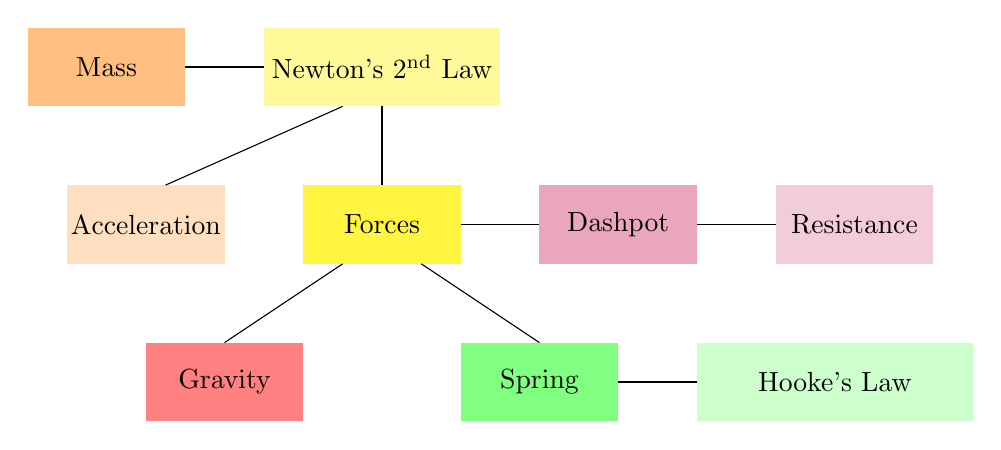
\begin{tikzpicture}
    \fill[color=orange!50!white] (-4.5,2) rectangle (-2.5,3) node[pos=.5] {\color{black}Mass};
%    \draw (-3.5,2) -- (-3.25,1);
    \fill[color=orange!25!white] (-4,1) rectangle (-2,0) node[pos=.5] {\color{black}Acceleration};
    \draw (-0.5,2) -- (-2.75,1);
    \draw (-2.5,2.5) -- (-1.5,2.5);
    \fill[color=yellow!40!white] (-1.5,2) rectangle (1.5,3) node[pos=.5] {\color{black}Newton's $2^{\rm nd}$ Law};
    \draw (0,1) -- (0,2);
  \fill[color=yellow!75!white] (-1,0) rectangle (1,1) node[pos=.5] {\color{black}Forces};
    \draw (-0.5,0) -- (-2,-1);
    \fill[color=red!50!white] (-1,-1) rectangle (-3,-2) node[pos=.5] {\color{black}Gravity};
    \draw (0.5,0) -- (2,-1);
    \fill[color=green!50!white] (3,-2) rectangle (1,-1) node[pos=.5] {\color{black}Spring};
    \draw (3,-1.5) -- (4,-1.5);
    \fill[color=green!20!white] (4,-2) rectangle (7.5,-1) node[pos=.5] {\color{black}Hooke's Law};
    \draw (1,0.5) -- (2,0.5);
    \fill[color=purple!35!white] (2,0) rectangle (4,1) node[pos=.5] {\color{black}Dashpot};  
    \draw (4,0.5) -- (5,0.5);
    \fill[color=purple!20!white] (5,0) rectangle (7,1) node[pos=.5] {\color{black}Resistance};  
\end{tikzpicture}
\end{center}
	
\end{example}


\paragraph{\emph{Step 3.}} Make assumptions

\begin{example}
In this step, we discuss the mind map we created and how we plan to address each of the boxes, or only some of the boxes. This will involve making assumptions and providing an explanation to the assumptions we make.

\begin{enumerate}
	\item As we described before the example, the plan is to use Newton's Second Law of Motion to describe the motion of the mass. This involves three quantities:
	\begin{itemize}
		\item mass: we assume that this is known to the modeller;
		\item acceleration: as we mentioned above, this is directly related to the position of the object. We have $y''(t)=$ acceleration, as long as we are assuming that the object is moving only vertically;
		\item forces: we need to find all the forces acting on the object and add them.
	\end{itemize}
\end{enumerate}

The forces acting on the object need to be discussed separately:
\begin{itemize}
	\item Gravity: we will go on a limb here and say that the force of the spring is much larger, so we will ignore this force;
	\item Spring: the force of the spring that acts on the mass follows Hooke's Law that says that the force is proportional to the extension/contraction of the spring. The constant of proportionality depends on the spring and we assume that it is known;
	\item Dashpot: the dashpot provides resistance. We will assume that it provides linear resistance to movement: the force is proportional to the velocity, with a proportionality constant that depends on the dashpot and is assumed to be known to the modeller.
\end{itemize}
	
\end{example}


\paragraph{\emph{Step 4.}} Construct a model

\begin{example}
We will start with Newton's Second Law of motion:
\begin{itemize}
	\item $m y''(t) = F(t)$ \\
\end{itemize}

and we will  add the different forces one by one:
\begin{itemize}
	\item Spring: the force of the spring is \quad $- k y(t)$; \hfill (you should check that the sign makes sense)
	\item Dashpot: the force of the dashpot is \quad $- \gamma y'(t)$. \hfill (you should also check the sign of this term) \\
\end{itemize}

Right now we have the following model:
$$
m y''(t) = -ky(t) - \gamma y'(t).
$$

\end{example}



\paragraph{\emph{Step 5.}} Model assessment

We'll skip this part here, but you should try to develop some tests to check the validity of the model we came up with.
Specifically, the fact that we ignored gravity should be checked to make sure that it doesn't affect our model too much.

\paragraph{\emph{Step 6.}} Putting it all together in a report

We'll skip this part here.





	\newpage

\begin{exercises}

	\begin{problist}
	
	\prob Consider a mountain with shape $y=f(x)$ a hiker who is climbing down the mountain with horizontal position $x(t)$. She starts at a peak of the mountain at $x_0=0$. As she climbs down the mountain, she notices that from her point-of-view, the rate of change of the slope of the mountain is decreasing linearly with time.
		The hiker also notices that her horizontal speed is constant.
	
		Model the hiker's position and the shape of the mountain.
	
	\prob 
	
	\begin{center}
		\includegraphics*[width=150pt]{images/module20-catenary.pdf}
	\end{center}

	\prob Model a ping pong ball travelling through the air.
	
	\begin{center}
		\includegraphics*[height=100pt]{images/module20-hotairballoon.pdf}
	\end{center}
	
	\prob Model an old TV floating or sinking in the ocean.
	
	\prob Model a container floating in the ocean with a leak that allows water to get inside.
	
	\prob Model a hot air balloon flying through the air.
	
	\prob Model the shape of a rope hanging between two poles.

	\begin{center}
		\includegraphics*[width=150pt]{images/module20-suspensionbridge.pdf}
	\end{center}

	\prob Model the shape of the cables of a suspension bridge.
	
	\prob Imagine a cylinder floating vertically partially submerged in a lake. Model the position of its top.
	
	\prob Model a ball rolling down a hill.
	
	\prob Model an electric circuit with a resistor, and inductor, and a capacitor in series.
	
	\prob Start with the Law of Conservation of Energy and assume a conservative force. Then show that you obtain Newton's Second Law of motion.
	
	\end{problist}
\end{exercises}

\end{module}



\begin{lesson}
	\Title{Modelling with Second-Order ODEs}

	\Heading{Objectives}
	\begin{itemize}
		\item Bla
	\end{itemize}
	
	\Heading{Motivation} 

\end{lesson}




\newpage

\question
	Here are some facts about laptop keys:

\begin{itemize}
\begin{minipage}{.4\textwidth}
\item[\color{Gray}(da)] Each key must also include some damping, so that it doesn't keep oscillating back and forth once pressed.

\item[\color{Gray}(di)] A typical letter key is 15mm$\times$15mm and when pressed has a maximum displacement of 0.5mm.

\item[\color{Gray}(fo)] On average, a person exerts the force of $42\,$N with one finger on a key.
\end{minipage}
\hfill
\begin{minipage}{.4\textwidth}
\item[\color{Gray}(gr)] Gravity is much weaker than the spring that keeps the key in place.

\item[\color{Gray}(hl)] Each key has a spring to make the key return to its original position after being pressed (Hooke's Law: ``the force is proportional to the extension'').

\item[\color{Gray}(lo)] Keys last 50 million presses on average.

\item[\color{Gray}(ve)] Keys can only move vertically.
\end{minipage}
\end{itemize}
	
	
\begin{parts}
	\item Model a laptop keypress.
	\item What happens if the damping system of the key is broken? What happens if the damping system is too strong? How strong should the damping system be?
	\item What happens to the key when the spring breaks?
\end{parts}









%%%%%%%%%%%%%%%%%%%%%%%%%%%%%%
%
%  MODULE - Second-Order Linear ODEs with Constant Coefficients
%
%%%%%%%%%%%%%%%%%%%%%%%%%%%%%%



\begin{module}{Second-Order Linear ODEs with Constant Coefficients}
	\label{2nd:solving}

	In this module you will learn
\begin{itemize}
	\item how to solve this type of ODEs
\end{itemize}

\hfill \\

In this module we will learn how to solve a specific type of Second-Order ODEs: linear second-order ODEs with constant coefficients. These equations have the form
$$
a y''(t)  + b y'(t) + c y(t) = f(t).
$$

\subsection{Homogeneous ODEs}

These are ODEs above with $f(t) \equiv 0$.
So we are trying to solve
$$
a y''(t)  + b y'(t) + c y(t) = 0.
$$

The main idea to solve these problems is the same as for systems: making an \emph{educated guess} that the solution should look like an exponential:
$$
y(t) = e^{rt},
$$
and we need to find which values of $r$ yield solutions.

We do that by plugging this formula for $y(t)$ into the ODE:
\begin{itemize}
	\item $y'(t) = r e^{rt}$
	\item $y''(t) = r^2 e^{rt}$
\end{itemize}

We get
$$
a r^2 e^{rt} + br e^{rt} + c e^{rt} = 0
\quad \Leftrightarrow \quad 
	a r^2 + br + c = 0.
$$

This equation for $r$ is called the \emph{characteristic equation}.

We know how to solve it:
$$
r = \frac{-b \pm \sqrt{b^2-4ac}}{2a}.
$$

That means that we have three possible cases.





\paragraph{\color{cyan}Two real distinct roots.} When $b^2-4ac > 0$, we have two possible values for $r$ that are real numbers: $r_1$ and $r_2$.

Then, similarly to what we did with systems of ODEs, we obtain two solutions
$$
y_1(t) = e^{r_1 t} \quad \text{ and } \quad y_2(t) = e^{r_2 t},
$$
and the general solution is
$$
y(t) = c_1 e^{r_1 t} + c_2 e^{r_2 t}.
$$

\begin{video}
\begin{itemize}
	\item \qrvideo{https://youtu.be/_8fcT95JV34}
	\item \qrvideo{https://youtu.be/nE_OnX8ulHA}
	\item \qrvideo{https://youtu.be/v1xKZOrGsVc}
\end{itemize}	
\end{video}



\paragraph{\color{cyan}Two complex roots.} When $b^2-4ac<0$, we have two possible values for $r$, but they are complex values:
$$
r_{\pm} = \alpha \pm i\beta.
$$
\begin{graybox}
What are the value of $\alpha$ and $\beta$?	
\end{graybox}

Then we have two solutions
$$
y_{+}(t) = e^{(\alpha+i\beta) t} \quad \text{ and } \quad y_{-}(t) = e^{(\alpha-i\beta) t},
$$
and the general solution is
$$
y(t) = a_1 e^{(\alpha+i\beta) t}  + a_2 e^{(\alpha-i\beta) t}.
$$

Just like we did with systems with complex eigenvalues, we prefer to write the solutions without complex numbers, so we expand it using Euler's formula to get
\begin{align*}
y(t) 	& = a_1 e^{(\alpha+i\beta) t}  + a_2 e^{(\alpha-i\beta) t} \\
		& = a_1 e^{\alpha t}e^{i\beta t}  + a_2 e^{\alpha t}e^{-i\beta t} \\
		& = a_1 e^{\alpha t} \big( \cos(\beta t) + i \sin(\beta t) \big)  + a_2 e^{\alpha t} \big( \cos(\beta t) - i \sin(\beta t) \big) \\
		& = (a_1+a_2)  \cos(\beta t)e^{\alpha t} + i (a_1-a_2)\sin(\beta t) e^{a\alpha t} \\
		& = c_1 \cos(\beta t)e^{\alpha t} + c_2\sin(\beta t) e^{\alpha t}
\end{align*}

\begin{graybox}
How do $c_1$ and $c_2$ depend on $a_1,a_2$?	
\end{graybox}

So another way to write the general solution is
$$
y(t) = c_1 \cos(\beta t)e^{\alpha t} + c_2\sin(\beta t) e^{\alpha t}.
$$


\begin{video}
\begin{itemize}
	\item \qrvideo{https://youtu.be/DORl6GMPtjM?t=396}
\end{itemize}	
\end{video}




\paragraph{\color{cyan}One real repeated root.} When $b^2-4ac=0$, then we are left with only one value for $r=-\frac{b}{2a}$.

We then have one solution
$$
y_1(t) = e^{-\frac{b}{2a}t}.
$$

\begin{example}
Consider the ODE 
$$
y''(t) + 2y'(t) + y(t) = 0.
$$	

To find the general solution, we assume that the solutions have the form $y(t) = e^{rt}$, which means that $r$ must satisfy
$$
r^2 +2r+1 = 0 
	\quad \Leftrightarrow \quad r=-1,
$$
so $y_1(t) = c_1 e^{-t}$.

Now can we solve this ODE with the following initial conditions?
\begin{itemize}
	\item $y(0)=2$ and $y'(0)=-2$.
	\item $y(0)=2$ and $y'(0)=1$.
\end{itemize}
\end{example}

This previous example, should give a good idea on why having one value for $r$ means that we are missing something. 
We need to find a second solution $y_2(t)$. \\


\begin{graybox}
If we want to find all the divisors of $42$, and we already know that $d_1=2$ is a divisor, then we can use the divisor $d_1$ we know to write 
$$
d_1 \cdot x = 42 
	\quad \Leftrightarrow\quad 2x = 42
	\quad \Leftrightarrow\quad x = 21,
$$
where $x$ is the product of all the other divisors.

We used the divisor we knew $d_1$ to obtain a simpler problem for the other divisors.
\end{graybox}


\subparagraph{\color{cyan}Reduction of Order.} The idea here is the same. We use the solution we found to try to obtain a simpler ODE for the other solution:
$$
y(t) = y_1(t) \cdot u(t),
$$
where $y(t)$ is the solution we are still missing, $y_1(t)$ is the solution we already found, and $u(t)$ is a function. If we find $u(t)$, then we find $y(t)$. We hope that the function $u(t)$ satisfies a simpler problem.

To do that, we need to plug the formula above for $y(t)$ into the original ODE. 

\begin{important}
You should do these calculations yourself.
Remember to use the product rule and to be careful not to make any mistakes.	

Also remember that we know the value of $r$.
\end{important}

We obtain
$$
u''(t) = 0
\quad \Leftrightarrow \quad u(t) = c_1 + c_2 t.
$$

This means that we found 
$$
y(t) = (c_1 + c_2 t) e^{rt}
\quad \Leftrightarrow \quad y(t) = \underbrace{c_1 e^{rt}}_{\substack{\rm previous \\ \text{solution } y_1(t)}} + c_2 t e^{rt}.
$$

The general solution is 
$$
y(t) = c_1 e^{rt} + c_2 t e^{rt},
$$
where $r = -\frac{b}{2a}$.


\begin{video}
\begin{itemize}
	\item \qrvideo{https://youtu.be/DORl6GMPtjM}
\end{itemize}	
\end{video}






\subsection{Non-Homogeneous ODEs}

We are trying to solve
\begin{equation}\tag{$\star$}\label{mod20:orig}
a y''(t)  + b y'(t) + c y(t) = f(t),
\end{equation}
where $f(t)$ is a known function. \\


\begin{important}
If $u(t)$ is the general solution of
\begin{equation}\tag{$H$}\label{mod20:hom}
ay''(t)+by'(t)+cy(t) = 0,
\end{equation}
and $v(t)$ satisfies
\begin{equation}\tag{\ref{mod20:orig}}
ay''(t)+by'(t)+cy(t) = f(t),
\end{equation}
then $y(t) = u(t) + v(t)$ gives the general solution of
$$
ay''(t)+by'(t)+cy(t) = f(t).
$$

This is a practice problem at the end of this module.
\end{important}


This means that to solve this ODE, we split the general solution into two parts
$$
y(t) = y_c(t) + y_p(t),
$$
where
\begin{itemize}
	\item $y_c(t)$ is called the \emph{complementary solution} and it is the general solution of the corresponding homogenous ODE \eqref{mod20:hom}. It is solved using the technique we studied above.
	\item $y_p(t)$ is called the \emph{particular solution} and it is one function that satisfies the original ODE \eqref{mod20:orig}.
\end{itemize}

\begin{important}
It may seem strange that to solve the original ODE, we need its solution, but what we are trying to do is find \emph{all possible solutions} of the original ODE.

To find all possible solutions of the original ODE, we require two things:
\begin{itemize}
	\item \emph{One} solution of the original ODE:  $y_p(t)$,
	\item and all possible solutions of the homogeneous ODE: $y_c(t)$.
\end{itemize}
\end{important}


We already know how to find the complementary solution, so we will focus our attention on finding one particular solution.

\paragraph{\color{cyan}Method of Undetermined Coefficients.} As you probably have gotten used to by now, this is a method of educated guess-and-check. \\

Let us look at the equation from a different point-of-view
\begin{align*}
a y''(t) + by'(t) + cy(t) & = f(t) \\
\substack{\displaystyle\text{linear combination of}\\\displaystyle\text{function and derivatives}} & = f(t)
\end{align*}
and remember that some functions don't change much when differentiated:
\begin{itemize}
	\item Exponentials $y=ce^{rt}$ don't change their form after differentiation $y'=cre^{rt} = de^{rt}$. They even keep the same exponential term.
	\item Polynomials don't change their form either: their derivative is also a polynomial, with lower degree.
	\item Cosines and Sines alternate between one and the other, so functions of the form $y=c_1 \sin(rt) + c_2\cos(rt)$ don't change after differentiation.
\end{itemize}


\begin{important}
This means that, if $f(t)$ is one of these types of function, then $y(t)$ must be of the same form.	
\end{important}

\begin{example}
Find a particular solution for the ODE
$$
y''  - 4y = 10 e^{3t} = (\text{constant}) \cdot (\text{exponential of } 3t).
$$	

Our candidate is
$$
y_p(t) = A e^{3t}.
$$

Now we need to find the constant $A$ by plugging it into the ODE:
$$
9 A e^{3t} - 4 \cdot A e^{3t} = 10 e^{3t}
\quad \Leftrightarrow \quad 
	A = 2,
$$
so $y_p(t) = 2 e^{3t}$ is a particular solution.
\end{example}


\begin{example}
Find a particular solution for the ODE
$$
y''  - 4y = 3t^2+2t = (\text{polynomial of degree 2}).
$$	

Our candidate is
$$
y_p(t) = At^2 + Bt + C.
$$

Now we need to find the constants $A, B, C$ by plugging the formula for $y_p$ into the ODE:
$$
2A - 4At^2 - 4B t - 4C = 3t^2+2t
\quad \Leftrightarrow \quad 
\begin{cases}
A = -\frac34 \\
B = -\frac12 \\
C = \frac{A}{2} = -\frac38.	
\end{cases}
$$
so $y_p(t) = -\frac34 t^2 - \frac{t}{2} - \frac38$ is a particular solution.
\end{example}

There are some more details to deal with when using this method that will be addressed in the core exercises.




\begin{video}
\begin{itemize}
	\item \qrvideo{https://youtu.be/CjZ0TfPnWVU}
	\item \qrvideo{https://youtu.be/ubdSxJ2nmVk}
	\item \qrvideo{https://youtu.be/YRvqem1n0nQ}
\end{itemize}	
\end{video}





	\begin{exercises}

	\begin{problist}

	\prob Find the complementary and particular solutions for the following ODEs
	\begin{enumerate}
		\item $y''-2y'-3y=3e^{2t}$
		\item $y''-2y'-3y=-3te^{-t}$
		\item $y''-9y=t^2e^{-3t}-6$
		\item $y''+2y'-8y=e^{-t}-2e^t$
		\item $y''-y'-6y=\sin(t)$
		\item $y''-y'-6y=\sin(t)+3e^{3t}$
		\item $y''+4y=(2t+1)\sin(t) + 4\cos(2t)$
		\item $y''+y=\cos(2t)+t^3$
		\item $y''-y'-2y=t\cos(t) - t\sin(t)$
		\item $y''+5y'+6y = 2e^{-2t}$
	\end{enumerate}



	\prob What is the form of the particular solution for the ODE
	\begin{multline*}
		y^{(6)} + y^{(5)} -5 y^{(4)} + 31 y'''-176y''+220y' \\
			= (3t-1)e^{2t} + t^3e^{-5t}\sin(3t) + (4t^2-2t) e^{-2t} \sin(3t),
	\end{multline*}
	knowing that 
	\begin{multline*}
		x^6 + x^5 - 5 x^4 + 31 x^3 - 176 x^2 + 220 x \\
			= \big((x^2+2)+9\big)*(x-2)^2*x*(x+5)\quad ?
	\end{multline*}

	\prob What is the form of the particular solution for the ODE
	\begin{multline*}
		y'''' - 4 y''' + 10y'' - 12 y' + 5y \\
			= t e^t + t^2 \cos(2t) - (2t+1) e^t \sin(t),
	\end{multline*}
	knowing that 
	\begin{multline*}
		x^4 - 4x^3 + 10 x^2 - 12 x + 5 \\
			= (x-1)^2 \big( (x-1)^2+4\big)\quad  ?
	\end{multline*}

	\prob Consider the ODE
	$$
	t^2 y''+ty'-9y = 0,
	$$
	and a solution $y_1(t) = t^3$.
	
	\begin{enumerate}
		\item Use the reduction of order technique to deduce the general solution to this problem.
		
		{\bf Hint.} You should find a second-order ODE for $u(t)$ without the term $u(t)$. So define $v(t) = u'(t)$ and solve the first-order ODE for $v(t)$.
		
		
			%	Solution: $tu'' + 7 u' = 0$ \\
			%	Define: $v = u'$ \\
			%	Solve: $tv' + 7 v = 0 \Rightarrow v = c_2 t^{-7}$ \\
			%	Then: $u = \int v = c_2 \int e^{t^2} dt + c_1$


		
		
		\item Find the solution with initial conditions $y(1)=1$ and $y'(1)=-3$.
		\item Find the solution with initial conditions $y(1)=1$ and $y'(1)=3$.
		\item Find the solution with initial conditions $y(1)=1$ and $y'(1)=0$.
	\end{enumerate}


	\prob Consider the ODE
	$$
	t^2 y'' - 3 t y' + 4 y = 0
	$$
	and a solution $y_1(t) = t^2$.
	
	\begin{enumerate}
		\item Use the reduction of order technique to deduce the general solution to this problem.
		
	
			%	Solution: $tu'' + 7 u' = 0$ \\
			%	Define: $v = u'$ \\
			%	Solve: $tv' + 7 v = 0 \Rightarrow v = c_2 t^{-7}$ \\
			%	Then: $u = \int v = c_2 \int e^{t^2} dt + c_1$
		
		\item Find the solution with initial conditions $y(1)=1$ and $y'(1)=2$.
		\item Find the solution with initial conditions $y(1)=0$ and $y'(1)=1$.
	\end{enumerate}



	
	\prob Consider the ODE $a y'' +by'+cy = f(t)$, with complementary solution $y_c(t) =c_1 y_1(t) + c_2 y_2(t)$ and particular solution $y_p(t)$.
	
	Consider also the initial conditions $y(0)=y_0$ and $y'(0)=v_0$.
	
	Show that there exist constants $c_1, c_2$ such that $y(t) = y_c(t) + y_p(t)$ solves the ODE with these initial conditions.
	
	\end{problist}
\end{exercises}

\end{module}



\begin{lesson}
	\Title{Second-Order Linear ODEs with Constant Coefficients}

	\Heading{Objectives}
	\begin{itemize}
		\item Bla
	\end{itemize}
	
	\Heading{Motivation} 

\end{lesson}




\newpage

\question
	Consider the ODE \quad $y''(t) -9y(t) = f(t)$.
\begin{parts}
	\item Find a complementary solution.
	\item Find a particular solution for $f(t) = 14 e^{-4t}$.
	\item Find a particular solution for $f(t) = 9 e^{-3t}$.
	\item Find a particular solution for $f(t) = 10\cos(t)$.
\end{parts}

\bookonlynewpage


\question
	Consider the ODE \quad $y''(t) -2y'(t)+5y(t) = f(t)$. %(roots $r = 1 \pm 2i$)
\begin{parts}
	\item Find a complementary solution.
	\item Find a particular solution for $f(t) = \sin(2t)e^t$.
	\item Find a particular solution for $f(t) = (4t+2)\sin(2t)e^t$.
\end{parts}




\bookonlynewpage


\question
	Consider the ODE \quad $y'' + 3y' = 3t$.
\begin{parts}
	\item Find the complementary solution.
	\item Find a particular solution.
	\item Find the solution that also satisfies
	$$ \begin{cases}
		y(0)=0 \\
		y'(0)=0
	\end{cases}$$
\end{parts}







%%%%%%%%%%%%%%%%%%%%%%%%%%%%%%
%
%  MODULE - Analysis of Higher Order ODEs
%
%%%%%%%%%%%%%%%%%%%%%%%%%%%%%%



\begin{module}{Analysis of Models with Higher Order ODEs}
	\label{2nd:analysis}

	In this module you will learn
\begin{itemize}
	\item different ways to analyze models with higher-order differential equations
\end{itemize}

\hfill \\



In this chapter, we have learned how to create models involving systems of ODEs and how to solve some special types of second-order ODEs.



In this module, we'll study one example using a few different methods.

\begin{example}
Consider the model we found earlier for a mass attached to a spring:

\begin{minipage}{0.85\textwidth}
\begin{itemize}
	\item $y(t)=$ vertical position of the mass, where $y=0$ is the position of the mass at rest
	\item $my''(t) = -k y(t) - \gamma y'(t)$
	\item $m,k,\gamma>0$ are constants for the mass, the stiffness of the spring, and the resistance of the dashpot.
\end{itemize}
\end{minipage}
\begin{minipage}{50pt}
\includegraphics*[height=100pt]{images/module16-spring-mass-dashpot.pdf}	
\end{minipage}
\end{example}

\hfill

\begin{center}
\textbf{\color{cyan}
Qualitative evolution of quantities
}
\end{center}


We can try to figure out how these quantities, $y(t)$, $y'(t)$, and $y''(t)$ are going to increase or decrease as time goes by. \\

Let us imagine that initially  \quad $y(0)=1, y'(0)=0$.

Then, at $t=0$, we have
$$
\begin{cases}
y(0)=1 \\
y'(0)=0 \\
y''(0)= -k < 0 & \text{ (so object is decelerating, meaning speed will become negative)}
\end{cases}
$$

This means that the object is decelerating, so we have two immediate consequences:
\begin{itemize}
	\item the speed will decrease and become negative
	\item the position will start decreasing
\end{itemize}

Once the speed is negative, we see another effect
$$
y''(t) = -k\underbrace{y(t)}_{\text{decreasing}} \underbrace{- \gamma y'(t)}_{\rm positive},
$$
so the acceleration is negative but approaching zero at time $t_1$:
$$
0=y''(t_1) = -ky(t_1) - \gamma y'(t_1)
\quad \Leftrightarrow \quad k y(t_1) = - \gamma y'(t_1)
$$

Let us summarize our results so far in a table:

\begin{graybox}
\begin{center}
\begin{tabular}{c||c|c|c|c|c|c|c|c}
$\pmb{t}$	& $0$ 		& 			& $t_1$ &  			& 			& 	&	& \hspace{1cm} $+\infty$ \\[5pt] \hline\hline
$\pmb{y}$ & $1$	& $ \searrow$	& $+$ &	$\searrow$ 	&	&  \hspace{0.5cm}	&  	& 	\\[5pt] \hline
$\pmb{y'}$ & $0$ &	$\searrow$	& $-$ & $\nearrow$ & 	&  	& &	\\[5pt] \hline
$\pmb{y''}$ & $-$		& $\nearrow$ & 0  & $\nearrow$  & 	& 	&  &	\\[5pt] \hline
\end{tabular}
\end{center}
\end{graybox}

The next milestone is:
$$
y(t_2)=0 \quad \text{ or } \quad y'(t_2)=0.
$$

If $y'(t_2)=0$ while $y(t_2)>0$, then 
$$
y''(t_2) = -ky(t_2) <0,
$$
which means that $y''$ would have had to decrease again, become zero and then negative, so there would have been another milestone before.
We deduce that the next milestone is
$$
y(t_2)=0
\quad \Leftrightarrow \quad	
	y''(t_2) = -\gamma y'(t_2) > 0.
$$

\begin{graybox}
\begin{center}
\begin{tabular}{c||c|c|c|c|c|c|c|c}
$\pmb{t}$	& $0$ 		& 			& $t_1$ &  			&	$t_2$& 	&$t_3$	& \hspace{1cm} $+\infty$ \\[5pt] \hline\hline
$\pmb{y}$ & $1$	& $ \searrow$	& $+$ &	$\searrow$ 	& $0$	&  $\searrow$ 	& $-$ 	& $\cdots$	\\[5pt] \hline
$\pmb{y'}$ & $0$ &	$\searrow$	& $-$ & $\nearrow$ & $-$	&  $\nearrow$	& $0$ &	$\cdots$ \\[5pt] \hline
$\pmb{y''}$ & $-$		& $\nearrow$ & 0  & $\nearrow$  & $+$ & $\nearrow$	& $+$ &	$ \cdots$ \\[5pt] \hline
\end{tabular}
\end{center}
\end{graybox}

We can continue this analysis to conclude that the position seems to cycle back and forth between positive and negative, like you would expect from a spring. \\

\begin{graybox}
In fact, this \emph{study is flawed}, since there is a possibility that the time $t_1$ never happens and the spring only approaches the state described without ever reaching it. This will happen for some configuration of the constants $m,k,\gamma$.
\end{graybox}




\hfill

\begin{center}
\textbf{\color{cyan}
Properties of the solutions
}
\end{center}



We learned earlier in the chapter how to solve this type of differential equations.

To solve them, we assume that solutions are of the form $y=e^{rt}$ and then find a characteristic equation for $r$:
$$
mr^2 = -k - \gamma r
\quad \Leftrightarrow \quad 
r = \frac{-\gamma \pm \sqrt{\gamma^2 - 4mk}}{2m}.
$$

Depending on the constants $m, k, \gamma$, we can have:
\begin{itemize}
	\item Two real distinct solutions 
	\item Two complex distinct solutions
	\item One repeated real solution
\end{itemize}

How do solutions behave in each case?
What kind of springs or dashpots imply each case?





\hfill

\begin{center}
\textbf{\color{cyan}
Limiting behaviour of the solutions
}
\end{center}


From the analysis done above, we see that the possible values for $r$ are either negative or when $r$ is complex, its real part is negative (why?).

This means that the solution will have the form
$$
y(t) = e^{(\text{negative constant}) t} \left[  a\cos(\alpha t) + b\sin(\beta t) + c\right],
$$
so 
$$
\lim_{t \to \infty} y(t) = 0.
$$

This means that the mass will slow down and eventually stop.


%\newpage
\hfill

\begin{center}
\textbf{\color{cyan}
Numerical approximations
}
\end{center}



In module \ref{ODE:approximation} we learned how to approximate solutions of first-order ODEs using Euler's Method.

We can extend that method to second-order ODEs, which we will leave as an exercise, and approximate the solution:

\begin{center}
\begin{tabular}{ccc}
\includegraphics*[width=125pt]{images/module21-approx-k2g5.png}
	& \includegraphics*[width=125pt]{images/module21-approx-k2g1.png}
	& \includegraphics*[width=125pt]{images/module21-approx-k2g0.png} \\
$k=2,\gamma=5$ 
	& $k=2,\gamma=1$ 
	& $k=2,\gamma=0$
\end{tabular}
\end{center}

These graphs also give us some intuition on how the solutions behave.

\begin{graybox}
You can access this simulation here:
\begin{itemize}
	\item \qrvideo{https://www.desmos.com/calculator/mufgdgku9w}
\end{itemize}	
\end{graybox}















	%\newpage 

\begin{exercises}

	\begin{center}
		\includegraphics*[height=100pt]{images/module20-hotairballoon.pdf}
	\end{center}

	\begin{problist}
	
	\prob Consider the model for a hot air balloon:
	\begin{itemize}
		\item $y(t) = $ altitude of the balloon;
		\item $y''(t) = \underbrace{-g}_{\rm gravity} + \underbrace{\big( g - 9 (y-1000) \big)}_{\rm lift} + p(t)$;
		\item $g=$ gravitational constant;
		\item $p(t)=$ passenger actions affecting the vertical acceleration of the balloon.
	\end{itemize}
	\begin{enumerate}
		\item What is the equilibrium altitude?
		\item How does the balloon behave without passenger actions?
		\item If the passenger actions are $p(t) = 6 \cos(\omega t)$, study how the constant $\omega$ changes the behaviour.
	\end{enumerate}
	

	

	\prob Consider the model for a cubic object floating/sinking in the ocean:
	\begin{itemize}
		\item $d(t) = $ depth of the object;
		\item $m d''(t)  = -mg - \gamma \big|d'(t)\big| d'(t) + A r^3$;
		\item $m=$ mass of the object;
		\item $r=$ length of one side of the object;
		\item $\gamma=$ water resistance constant;
		\item $A=$ buoyancy constant (density of water minus density of object).
	\end{itemize}

	\begin{enumerate}
		\item Does the object float or sink? 
		\item What is the terminal vertical velocity of the object?
		\item Assume the constants $r=\frac12$m, $m=30$kg, $\gamma =1$kg/m, $A=300 \cdot 2^3$kg/(ms)$^2$, and approximate $g\approx 10$m/s$^2$. Assume that the initial depth of the object is 0m (the surface of the ocean). 
			
			What is the object's terminal velocity?
			Will it reach the bottom of the ocean?
	\end{enumerate}
	
	
	\begin{center}
		\includegraphics*[width=50pt]{images/module22-spring-mass.pdf}
	\end{center}

	
	\prob Consider the following model for a spring-mass system:
	\begin{itemize}
		\item $y(t) = $ position of the mass;
		\item $y''(t)  = -ky(t) + f(t)$;
		\item $k=$ stiffness of the spring;
		\item $f(t)=$ extra force on the mass.
	\end{itemize}

	\begin{enumerate}
		\item How does the spring behave when there is no external force?
		\item Assume $k=9$. How does the spring behave when the external force is $f(t)=\cos(4t)$?
		\item Assume $k=9$. How does the spring behave when the external force is $f(t)=\cos(3t)$?
		\item Assume $k=9$. How does the spring behave when the external force is $f(t)=\cos(2.95t)$?
	\end{enumerate}
	
	
	\hspace{-1cm}\includegraphics*[width=250pt]{images/chap4-xkcd.png}
	

	
	\prob Explain how the initial statement of the comic makes sense.
		
	\end{problist}
\end{exercises}
\end{module}



\begin{lesson}
	\Title{Analysis of Models with Higher Order ODEs}

	\Heading{Objectives}
	\begin{itemize}
		\item Bla
	\end{itemize}
	
	\Heading{Motivation} 

\end{lesson}




\newpage

\question

